% Choose one to switch between slides and handout
\documentclass[]{beamer}
%\documentclass[handout]{beamer}

% Video Meta Data
\title{Bitcoin, Blockchain and Cryptoassets}
\subtitle{Signature Hash Types}
\author{Prof. Dr. Fabian Schär}
\institute{University of Basel}

% Config File
% Packages
\usepackage[utf8]{inputenc}
\usepackage{hyperref}
\usepackage{gitinfo2}
\usepackage{tikz}
\usepackage{amsmath}
\usepackage{bibentry}
\usepackage{xcolor}
\usepackage{colortbl} % Add colour to LaTeX tables
\usepackage{caption}
\usepackage[export]{adjustbox}
\usepackage{pgfplots} \pgfplotsset{compat = 1.17}

% Color Options
\definecolor{highlight}{rgb}{0.65,0.84,0.82}
\definecolor{focus}{rgb}{0.72, 0, 0}

% Beamer Template Options
\beamertemplatenavigationsymbolsempty
\setbeamertemplate{footline}[frame number]
\setbeamercolor{structure}{fg=black}
\setbeamercolor{footline}{fg=black}
\setbeamercolor{title}{fg=black}
\setbeamercolor{frametitle}{fg=black}
\setbeamercolor{item}{fg=black}
\setbeamercolor{}{fg=black}
\setbeamercolor{bibliography item}{fg=black}
\setbeamercolor*{bibliography entry title}{fg=black}
\setbeamertemplate{items}[square]
\setbeamertemplate{enumerate items}[default]
\captionsetup[figure]{labelfont={color=black},font={color=black}}
\captionsetup[table]{labelfont={color=black},font={color=black}}

\setbeamertemplate{bibliography item}{\insertbiblabel}

% Link Icon Command
\newcommand{\link}{%
    \tikz[x=1.2ex, y=1.2ex, baseline=-0.05ex]{%
        \begin{scope}[x=1ex, y=1ex]
            \clip (-0.1,-0.1)
                --++ (-0, 1.2)
                --++ (0.6, 0)
                --++ (0, -0.6)
                --++ (0.6, 0)
                --++ (0, -1);
            \path[draw,
                line width = 0.5,
                rounded corners=0.5]
                (0,0) rectangle (1,1);
        \end{scope}
        \path[draw, line width = 0.5] (0.5, 0.5)
            -- (1, 1);
        \path[draw, line width = 0.5] (0.6, 1)
            -- (1, 1) -- (1, 0.6);
        }
    }

% Read Git Data from Github Actions Workflow
% Defaults to gitinfo2 for local builds
\IfFileExists{gitInfo.txt}
	{\input{gitInfo.txt}}
	{
		\newcommand{\gitRelease}{(Local Release)}
		\newcommand{\gitSHA}{\gitHash}
		\newcommand{\gitDate}{\gitAuthorIsoDate}
	}

% Custom Titlepage
\defbeamertemplate*{title page}{customized}[1][]
{
  \vspace{-0cm}\hfill
\includegraphics[width=2.5cm]{../config/logo_cif}
  
\includegraphics[width=1.9cm]{../config/seal_wwz}
  \\ \vspace{2em}
  \usebeamerfont{title}\textbf{\inserttitle}\par
  \usebeamerfont{title}\usebeamercolor[fg]{title}\insertsubtitle\par  \vspace{1.5em}
  \small\usebeamerfont{author}\insertauthor\par
  \usebeamerfont{author}\insertinstitute\par \vspace{2em}
  \usebeamercolor[fg]{titlegraphic}\inserttitlegraphic
    \tiny \noindent \texttt{Release Ver.: \gitRelease}\\ 
    \texttt{Version Hash: \gitSHA}\\
    \texttt{Version Date: \gitDate}\\ \vspace{1em}
  \link \href{https://github.com/cifunibas/Bitcoin-Blockchain-Cryptoassets/blob/main/slides/intro.pdf}
  {Get most recent version}\\
  \link \href{https://github.com/cifunibas/Bitcoin-Blockchain-Cryptoassets/blob/main/slides/intro.pdf}
  {Watch video lecture}\\ \vspace{1em}
  License: \texttt{Creative Commons Attribution-NonCommercial-ShareAlike 4.0 International}\\\vspace{2em}
  
\includegraphics[width = 1.2cm]{../config/license}
}

% tikzlibraries
\usetikzlibrary{decorations.pathreplacing}
\usetikzlibrary{decorations.markings}
\usetikzlibrary{positioning}

%caption font
\captionsetup{font=footnotesize}


%%%%%%%%%%%%%%%%%%%%%%%%%%%%%%%%%%%%%%%%%%%%%%
%%%%%%%%%%%%%%%%%%%%%%%%%%%%%%%%%%%%%%%%%%%%%%
\begin{document}

\thispagestyle{empty}
\begin{frame}[noframenumbering]
	\titlepage
\end{frame}

\begin{frame}{Signature}
Network participants exchange signed transaction messages.\\ \vspace{1em}
	
In most cases, they sign all in- and outputs. However, in some cases, there may be a need for a more flexible approach. As such, there is the option to only sign certain in- and outputs.\\
	\vspace{1.5em}
	\uncover<2->{$\rightarrow$ \texttt{SIGHASH} types enable this.}
\end{frame}

\begin{frame}{SIGHASH Types Overview}
	There are three base \texttt{SIGHASH} types plus the \texttt{ANYONECANPAY} modifier:\\
	\vspace{1.5em}
	\scriptsize
	\begin{tabular}{l|ll}
		& All inputs & Only your input\\
		\hline
	All outputs & \texttt{SIGHASH\_ALL} & \texttt{SIGHASH\_ALL|SIGHASH\_ANYONECANPAY}\\
	Single output & \texttt{SIGHASH\_SINGLE} & \texttt{SIGHASH\_SINGLE|SIGHASH\_ANYONECANPAY}\\
	No outputs & \texttt{SIGHASH\_NONE} & \texttt{SIGHASH\_NONE|SIGHASH\_ANYONECANPAY}
	\end{tabular}
\end{frame}

\begin{frame}{\texttt{SIGHASH\_ALL}}
	\begin{figure}
		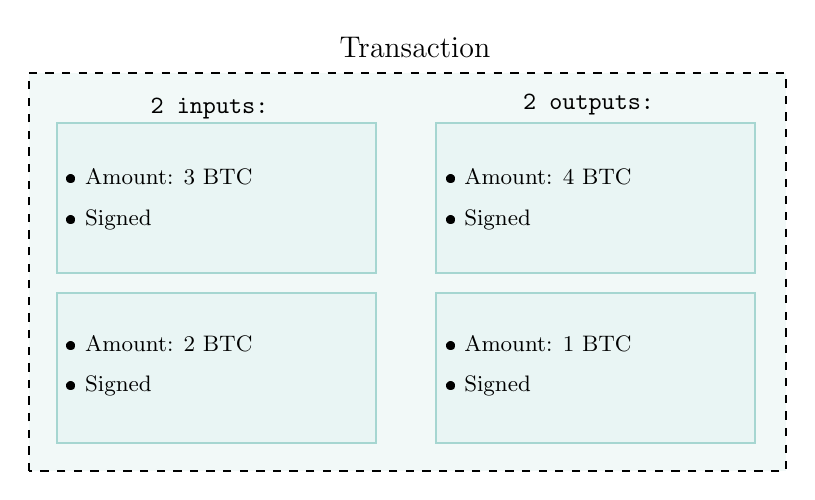
\begin{tikzpicture}[scale=0.9, every node/.style={scale=0.9}]
    
        \filldraw[yshift=-0.05cm, xshift=0.1cm,color = highlight!15, thick, draw=black, dashed] (-4,-6.4) rectangle ++(304pt,160pt);
        
    \draw[color=black] plot (1.55,-0.2) node [below]
    {\large{{Transaction}}};
    
    % Inputs
    \draw[color=black] plot (-1.35,-1.6) node[above] {\texttt{2 inputs:}};
    
    % top left
    \filldraw[yshift=-0.05cm, xshift=0.1cm,color = highlight!25, thick, draw=highlight] (-3.6,-3.6) rectangle ++(128pt,60pt);
    \draw[color=black] plot (-3.5,-2.3) node[right] {\small{\textbullet{} Amount: 3 BTC}};
%    \draw[color=black] plot (-3.5,-2.6)   node[right] {\small{\textbullet{} Anyone's input}};
    \draw[color=black] plot (-3.5,-2.9)   node[right] {\small{\textbullet{} Signed}};
    
    % bottom left
    \filldraw[yshift=-0.05cm, xshift=0.1cm,color = highlight!25, thick, draw=highlight] (-3.6,-6) rectangle ++(128pt,60pt);
    \draw[color=black] plot (-3.5,-4.65) node[right] {\small{\textbullet{} Amount: 2 BTC}};
%    \draw[color=black] plot (-3.5,-4.95)   node[right] {\small{\textbullet{} Anyone's input}};
    \draw[color=black] plot (-3.5,-5.25)   node[right] {\small{\textbullet{} Signed}};

	% Outputs
    \draw[color=black] plot (4,-1.55)   node[above] {\texttt{2 outputs:}};

	% top right
	\filldraw[yshift=-0.05cm, xshift=0.1cm,color = highlight!25, thick, draw=highlight] (1.75,-3.6) rectangle ++(128pt,60pt);
	\draw[color=black] plot (1.85,-2.3)   node[right] {\small{\textbullet{} Amount: 4 BTC}};
%    \draw[color=black] plot (1.85,-2.6)   node[right] {\small{\textbullet{} Unlocking condition}};
    \draw[color=black] plot (1.85,-2.9)   node[right] {\small{\textbullet{} Signed}};

	% bottom right
    \filldraw[yshift=-0.05cm, xshift=0.1cm,color = highlight!25, thick, draw=highlight] (1.75,-6) rectangle ++(128pt,60pt);
    \draw[color=black] plot (1.85,-4.65)   node[right] {\small{\textbullet{} Amount: 1 BTC}};
%    \draw[color=black] plot (1.85,-4.95)   node[right] {\small{\textbullet{} Unlocking condition}};
    \draw[color=black] plot (1.85,-5.25)   node[right] {\small{\textbullet{} Signed}};

\end{tikzpicture}
	\end{figure}
	\begin{itemize}
		\item Default value
		\item Signs all inputs and outputs.
		\item Modified inputs or outputs invalidate the signature.
	\end{itemize}
\end{frame}

\begin{frame}{\texttt{SIGHASH\_SINGLE}}
	\begin{figure}
		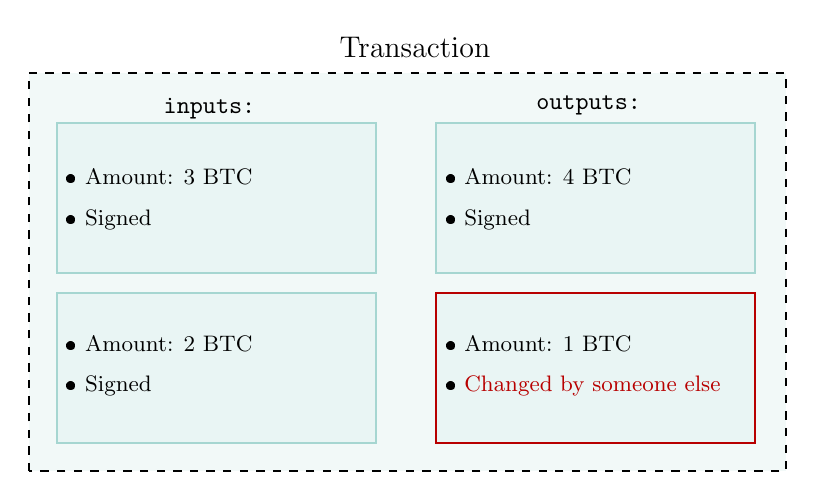
\begin{tikzpicture}[scale=0.9, every node/.style={scale=0.9}]
    
        \filldraw[yshift=-0.05cm, xshift=0.1cm,color = highlight!15, thick, draw=black, dashed] (-4,-6.4) rectangle ++(304pt,160pt);
        
    \draw[color=black] plot (1.55,-0.2) node [below]
    {\large{{Transaction}}};
    
    % Inputs
    \draw[color=black] plot (-1.35,-1.6) node[above] {\texttt{inputs:}};
    
    % top left
    \filldraw[yshift=-0.05cm, xshift=0.1cm,color = highlight!25, thick, draw=highlight] (-3.6,-3.6) rectangle ++(128pt,60pt);
    \draw[color=black] plot (-3.5,-2.3) node[right] {\small{\textbullet{} Amount: 3 BTC}};
%    \draw[color=black] plot (-3.5,-2.6)   node[right] {\small{\textbullet{} Anyone's input}};
    \draw[color=black] plot (-3.5,-2.9)   node[right] {\small{\textbullet{} Signed}};
    
    % bottom left
    \filldraw[yshift=-0.05cm, xshift=0.1cm,color = highlight!25, thick, draw=highlight] (-3.6,-6) rectangle ++(128pt,60pt);
    \draw[color=black] plot (-3.5,-4.65) node[right] {\small{\textbullet{} Amount: 2 BTC}};
%    \draw[color=black] plot (-3.5,-4.95)   node[right] {\small{\textbullet{} Anyone's input}};
    \draw[color=black] plot (-3.5,-5.25)   node[right] {\small{\textbullet{} Signed}};

	% Outputs
    \draw[color=black] plot (4,-1.55)   node[above] {\texttt{outputs:}};

	% top right
	\filldraw[yshift=-0.05cm, xshift=0.1cm,color = highlight!25, thick, draw=highlight] (1.75,-3.6) rectangle ++(128pt,60pt);
	\draw[color=black] plot (1.85,-2.3)   node[right] {\small{\textbullet{} Amount: 4 BTC}};
%    \draw[color=black] plot (1.85,-2.6)   node[right] {\small{\textbullet{} Unlocking condition}};
    \draw[color=black] plot (1.85,-2.9)   node[right] {\small{\textbullet{} Signed}};

	% bottom right
    \filldraw[yshift=-0.05cm, xshift=0.1cm,color = highlight!25, thick, draw=focus] (1.75,-6) rectangle ++(128pt,60pt);
    \draw[color=black] plot (1.85,-4.65)   node[right] {\small{\textbullet{} Amount: 1 BTC}};
%    \draw[color=black] plot (1.85,-4.95)   node[right] {\small{\textbullet{} Unlocking condition}};
    \draw[color=black] plot (1.85,-5.25)   node[right] {\small{\textbullet{} Unsigned}};
    
    \uncover<2->{
     	\filldraw[yshift=-0.05cm, xshift=0.1cm,color = highlight!25, thick, draw=focus] (1.75,-6) rectangle ++(128pt,60pt);
    	\draw[color=black] plot (1.85,-4.65)   node[right] {\small{\textbullet{} Amount: 1 BTC}};
%    	\draw[color=black] plot (1.85,-4.95)   node[right] {\small{\textbullet{} Unlocking condition}};
    	\draw[color=black] plot (1.85,-5.25)   node[right] {\small{\textbullet{} \textcolor{focus}{Changed by someone else}}};
    }
    
\end{tikzpicture}
	
	\end{figure}
	\begin{itemize}
		\item Signs all inputs and \emph{one} output only.
		\item Modified inputs or the modification of the signed output invalidate the signature.
		\item Other people can change any of the unsigned outputs.
	\end{itemize}
\end{frame}

\begin{frame}{\texttt{SIGHASH\_NONE}}
	\begin{figure}
		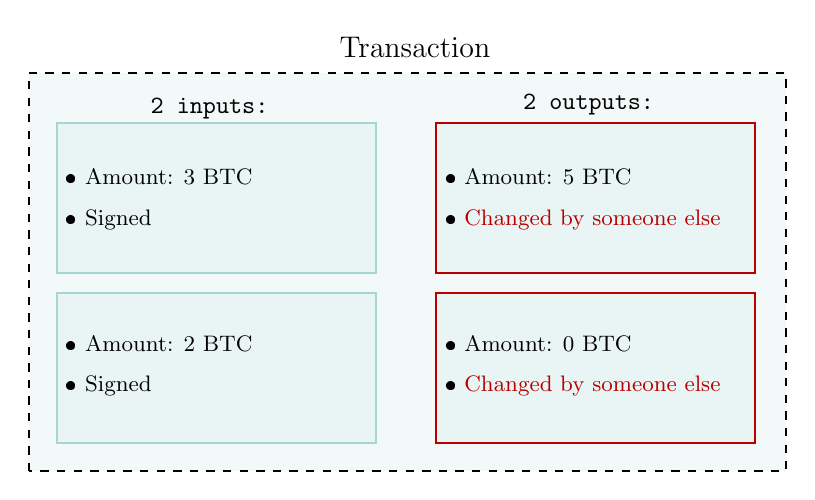
\begin{tikzpicture}[scale=0.9, every node/.style={scale=0.9}]
    
        \filldraw[yshift=-0.05cm, xshift=0.1cm,color = highlight!15, thick, draw=black, dashed] (-4,-6.4) rectangle ++(304pt,160pt);
        
    \draw[color=black] plot (1.55,-0.2) node [below]
    {\large{{Transaction}}};
    
    % Inputs
    \draw[color=black] plot (-1.35,-1.6) node[above] {\texttt{2 inputs:}};
    
    % top left
    \filldraw[yshift=-0.05cm, xshift=0.1cm,color = highlight!25, thick, draw=highlight] (-3.6,-3.6) rectangle ++(128pt,60pt);
    \draw[color=black] plot (-3.5,-2.3) node[right] {\small{\textbullet{} Amount: 3 BTC}};
%    \draw[color=black] plot (-3.5,-2.6)   node[right] {\small{\textbullet{} Anyone's input}};
    \draw[color=black] plot (-3.5,-2.9)   node[right] {\small{\textbullet{} Signed}};
    
    % bottom left
    \filldraw[yshift=-0.05cm, xshift=0.1cm,color = highlight!25, thick, draw=highlight] (-3.6,-6) rectangle ++(128pt,60pt);
    \draw[color=black] plot (-3.5,-4.65) node[right] {\small{\textbullet{} Amount: 2 BTC}};
%    \draw[color=black] plot (-3.5,-4.95)   node[right] {\small{\textbullet{} Anyone's input}};
    \draw[color=black] plot (-3.5,-5.25)   node[right] {\small{\textbullet{} Signed}};

	% Outputs
    \draw[color=black] plot (4,-1.55)   node[above] {\texttt{2 outputs:}};

	% top right
	\filldraw[yshift=-0.05cm, xshift=0.1cm,color = highlight!25, thick, draw=focus] (1.75,-3.6) rectangle ++(128pt,60pt);
	\draw[color=black] plot (1.85,-2.3)   node[right] {\small{\textbullet{} Amount: 4 BTC}};
%    \draw[color=black] plot (1.85,-2.6)   node[right] {\small{\textbullet{} Unlocking condition}};
    \draw[color=black] plot (1.85,-2.9)   node[right] {\small{\textbullet{} Unsigned}};

	% bottom right
    \filldraw[yshift=-0.05cm, xshift=0.1cm,color = highlight!25, thick, draw=focus] (1.75,-6) rectangle ++(128pt,60pt);
    \draw[color=black] plot (1.85,-4.65)   node[right] {\small{\textbullet{} Amount: 1 BTC}};
%    \draw[color=black] plot (1.85,-4.95)   node[right] {\small{\textbullet{} Unlocking condition}};
    \draw[color=black] plot (1.85,-5.25)   node[right] {\small{\textbullet{} Unsigned}};
    
    \uncover<2->{
    % top right
    \filldraw[yshift=-0.05cm, xshift=0.1cm,color = highlight!25, thick, draw=focus] (1.75,-3.6) rectangle ++(128pt,60pt);
	\draw[color=black] plot (1.85,-2.3)   node[right] {\small{\textbullet{} Amount: 5 BTC}};
%   \draw[color=black] plot (1.85,-2.6)   node[right] {\small{\textbullet{} Unlocking condition}};
    \draw[color=black] plot (1.85,-2.9)   node[right] {\small{\textbullet{} \textcolor{focus}{Changed by someone else}}};
    }
    
    \uncover<2->{
    	\filldraw[yshift=-0.05cm, xshift=0.1cm,color = highlight!25, thick, draw=focus] (1.75,-6) rectangle ++(128pt,60pt);
    	\draw[color=black] plot (1.85,-4.65)   node[right] {\small{\textbullet{} Amount: 0 BTC}};
%    	\draw[color=black] plot (1.85,-4.95)   node[right] {\small{\textbullet{} Unlocking condition}};
    	\draw[color=black] plot (1.85,-5.25)   node[right] {\small{\textbullet{} \textcolor{focus}{Changed by someone else}}};
    }

\end{tikzpicture}	
	\end{figure}
	\begin{itemize}
		\item Signs all inputs but \emph{none} of the outputs.
		\item Anyone can freely modify the unlocking conditions.
	\end{itemize}
\end{frame}

\begin{frame}{\texttt{SIGHASH\_ALL|SIGHASH\_ANYONECANPAY}}
	\begin{figure}
		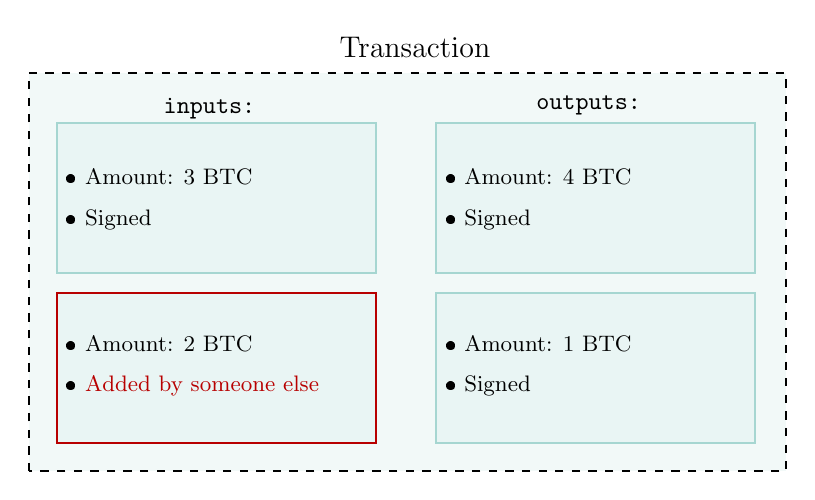
\begin{tikzpicture}[scale=0.9, every node/.style={scale=0.9}]
    
        \filldraw[yshift=-0.05cm, xshift=0.1cm,color = highlight!15, thick, draw=black, dashed] (-4,-6.4) rectangle ++(304pt,160pt);
        
    \draw[color=black] plot (1.55,-0.2) node [below]
    {\large{{Transaction}}};
    
    % Inputs
    \draw[color=black] plot (-1.35,-1.6) node[above] {\texttt{inputs:}};
    
    % top left
    \filldraw[yshift=-0.05cm, xshift=0.1cm,color = highlight!25, thick, draw=highlight] (-3.6,-3.6) rectangle ++(128pt,60pt);
    \draw[color=black] plot (-3.5,-2.3) node[right] {\small{\textbullet{} Amount: 3 BTC}};
%    \draw[color=black] plot (-3.5,-2.6)   node[right] {\small{\textbullet{} Anyone's input}};
    \draw[color=black] plot (-3.5,-2.9)   node[right] {\small{\textbullet{} Signed}};
    
    % bottom left
    \uncover<2>{
    	\filldraw[yshift=-0.05cm, xshift=0.1cm,color = highlight!25, thick, draw=focus] (-3.6,-6) rectangle ++(128pt,60pt);
    	\draw[color=black] plot (-3.5,-4.65) node[right] {\small{\textbullet{} Amount: 0.5 BTC}};
%    \draw[color=black] plot (-3.5,-4.95)   node[right] {\small{\textbullet{} Anyone's input}};
    	\draw[color=black] plot (-3.5,-5.25)   node[right] {\small{\textbullet{} \textcolor{focus}{Added by someone else}}};
    }
    
    \uncover<3>{
    	\filldraw[yshift=-0.05cm, xshift=0.1cm,color = highlight!25, thick, draw=focus] (-3.6,-6) rectangle ++(128pt,60pt);
    	\draw[color=black] plot (-3.5,-4.65) node[right] {\small{\textbullet{} Amount: 2 BTC}};
%    \draw[color=black] plot (-3.5,-4.95)   node[right] {\small{\textbullet{} Anyone's input}};
    	\draw[color=black] plot (-3.5,-5.25)   node[right] {\small{\textbullet{} \textcolor{focus}{Added by someone else}}};
    }

	% Outputs
    \draw[color=black] plot (4,-1.55)   node[above] {\texttt{outputs:}};

	% top right
	\filldraw[yshift=-0.05cm, xshift=0.1cm,color = highlight!25, thick, draw=highlight] (1.75,-3.6) rectangle ++(128pt,60pt);
	\draw[color=black] plot (1.85,-2.3)   node[right] {\small{\textbullet{} Amount: 4 BTC}};
%    \draw[color=black] plot (1.85,-2.6)   node[right] {\small{\textbullet{} Unlocking condition}};
    \draw[color=black] plot (1.85,-2.9)   node[right] {\small{\textbullet{} Signed}};
    
    % bottom right
    % bottom right
    \filldraw[yshift=-0.05cm, xshift=0.1cm,color = highlight!25, thick, draw=highlight] (1.75,-6) rectangle ++(128pt,60pt);
    \draw[color=black] plot (1.85,-4.65)   node[right] {\small{\textbullet{} Amount: 1 BTC}};
    \draw[color=black] plot (1.85,-5.25)   node[right] {\small{\textbullet{} Signed}};

\end{tikzpicture}

	\end{figure}
	\begin{itemize}
		\item Signs only the signer's inputs and all outputs.
		\item Anyone can add or remove other inputs.
		\item E.g.\ crowdfunding campaign
	\end{itemize}
\end{frame}

\begin{frame}{\texttt{SIGHASH\_SINGLE|SIGHASH\_ANYONECANPAY}}
	\begin{figure}
		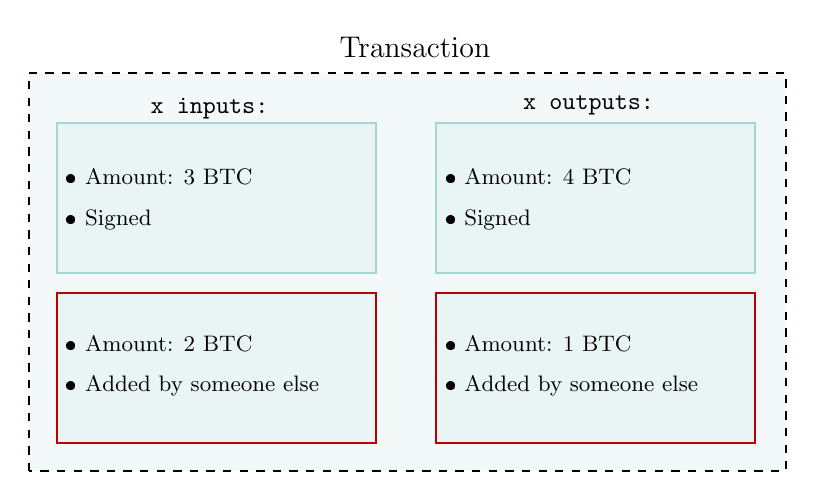
\begin{tikzpicture}[scale=0.9, every node/.style={scale=0.9}]
    
        \filldraw[yshift=-0.05cm, xshift=0.1cm,color = highlight!15, thick, draw=black, dashed] (-4,-6.4) rectangle ++(304pt,160pt);
        
    \draw[color=black] plot (1.55,-0.2) node [below]
    {\large{{Transaction}}};
    
    % Inputs
    \draw[color=black] plot (-1.35,-1.6) node[above] {\texttt{x inputs:}};
    
    % top left
    \filldraw[yshift=-0.05cm, xshift=0.1cm,color = highlight!25, thick, draw=highlight] (-3.6,-3.6) rectangle ++(128pt,60pt);
    \draw[color=black] plot (-3.5,-2.3) node[right] {\small{\textbullet{} Amount: 3 BTC}};
%    \draw[color=black] plot (-3.5,-2.6)   node[right] {\small{\textbullet{} Anyone's input}};
    \draw[color=black] plot (-3.5,-2.9)   node[right] {\small{\textbullet{} Signed}};
    
    % bottom left
    \uncover<2->{
    	\filldraw[yshift=-0.05cm, xshift=0.1cm,color = highlight!25, thick, draw=focus] (-3.6,-6) rectangle ++(128pt,60pt);
    	\draw[color=black] plot (-3.5,-4.65) node[right] {\small{\textbullet{} Amount: 2 BTC}};
%    \draw[color=black] plot (-3.5,-4.95)   node[right] {\small{\textbullet{} Anyone's input}};
    	\draw[color=black] plot (-3.5,-5.25)   node[right] {\small{\textbullet{} Added by someone else}};
    }
    
	% Outputs
    \draw[color=black] plot (4,-1.55)   node[above] {\texttt{x outputs:}};

	% top right
	\filldraw[yshift=-0.05cm, xshift=0.1cm,color = highlight!25, thick, draw=highlight] (1.75,-3.6) rectangle ++(128pt,60pt);
	\draw[color=black] plot (1.85,-2.3)   node[right] {\small{\textbullet{} Amount: 4 BTC}};
%    \draw[color=black] plot (1.85,-2.6)   node[right] {\small{\textbullet{} Unlocking condition}};
    \draw[color=black] plot (1.85,-2.9)   node[right] {\small{\textbullet{} Signed}};
    
    \uncover<2->{
    % bottom right
    \filldraw[yshift=-0.05cm, xshift=0.1cm,color = highlight!25, thick, draw=focus] (1.75,-6) rectangle ++(128pt,60pt);
    \draw[color=black] plot (1.85,-4.65)   node[right] {\small{\textbullet{} Amount: 1 BTC}};
%    \draw[color=black] plot (1.85,-4.95)   node[right] {\small{\textbullet{} Unlocking condition}};
    \draw[color=black] plot (1.85,-5.25)   node[right] {\small{\textbullet{} Added by someone else}};
    }

\end{tikzpicture}	
	\end{figure}
	\begin{itemize}
		\item Signs only the signer's input and \emph{one} output.
		\item Other people are free to add or remove additional inputs and outputs.\\
		\item Any change to the signer's part of the transaction will invalidate the signature.	
	\end{itemize}
\end{frame}

\begin{frame}{\texttt{SIGHASH\_NONE|SIGHASH\_ANYONECANPAY}}
	\begin{figure}
		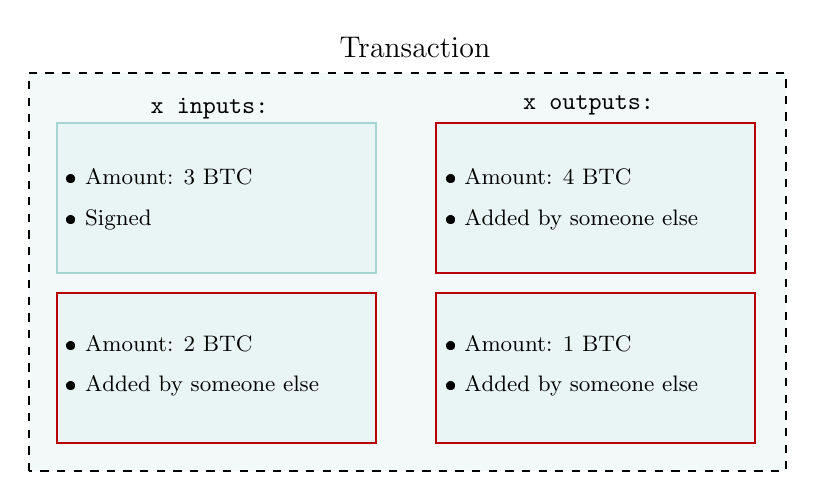
\begin{tikzpicture}[scale=0.9, every node/.style={scale=0.9}]
    
        \filldraw[yshift=-0.05cm, xshift=0.1cm,color = highlight!15, thick, draw=black, dashed] (-4,-6.4) rectangle ++(304pt,160pt);
        
    \draw[color=black] plot (1.55,-0.2) node [below]
    {\large{{Transaction}}};
    
    % Inputs
    \draw[color=black] plot (-1.35,-1.6) node[above] {\texttt{x inputs:}};
    
    % top left
    \filldraw[yshift=-0.05cm, xshift=0.1cm,color = highlight!25, thick, draw=highlight] (-3.6,-3.6) rectangle ++(128pt,60pt);
    	\draw[color=black] plot (-3.5,-2.3) node[right] {\small{\textbullet{} Amount: 3 BTC}};
%    	\draw[color=black] plot (-3.5,-2.6)   node[right] {\small{\textbullet{} Anyone's input}};
    	\draw[color=black] plot (-3.5,-2.9)   node[right] {\small{\textbullet{} Signed}};
    
    % bottom left
    \uncover<3->{
    	\filldraw[yshift=-0.05cm, xshift=0.1cm,color = highlight!25, thick, draw=focus] (-3.6,-6) rectangle ++(128pt,60pt);
    	\draw[color=black] plot (-3.5,-4.65) node[right] {\small{\textbullet{} Amount: 2 BTC}};
%    	\draw[color=black] plot (-3.5,-4.95)   node[right] {\small{\textbullet{} Anyone's input}};
    	\draw[color=black] plot (-3.5,-5.25)   node[right] {\small{\textbullet{} Added by someone else}};
    }
    
	% Outputs
    \draw[color=black] plot (4,-1.55)   node[above] {\texttt{x outputs:}};

	% top right
	\uncover<2>{\filldraw[yshift=-0.05cm, xshift=0.1cm,color = highlight!25, thick, draw=focus] (1.75,-3.6) rectangle ++(128pt,60pt);
		\draw[color=black] plot (1.85,-2.3)   node[right] {\small{\textbullet{} Amount: 3 BTC}};
%    	\draw[color=black] plot (1.85,-2.6)   node[right] {\small{\textbullet{} Unlocking condition}};
    	\draw[color=black] plot (1.85,-2.9)   node[right] {\small{\textbullet{} Added by someone else}};}
	
	\uncover<3->{
		\filldraw[yshift=-0.05cm, xshift=0.1cm,color = highlight!25, thick, draw=focus] (1.75,-3.6) rectangle ++(128pt,60pt);
		\draw[color=black] plot (1.85,-2.3)   node[right] {\small{\textbullet{} Amount: 4 BTC}};
%    	\draw[color=black] plot (1.85,-2.6)   node[right] {\small{\textbullet{} Unlocking condition}};
    	\draw[color=black] plot (1.85,-2.9)   node[right] {\small{\textbullet{} Added by someone else}};
    }


	% bottom right
	\uncover<3->{
    	\filldraw[yshift=-0.05cm, xshift=0.1cm,color = highlight!25, thick, draw=focus] (1.75,-6) rectangle ++(128pt,60pt);
    	\draw[color=black] plot (1.85,-4.65)   node[right] {\small{\textbullet{} Amount: 1 BTC}};
%    	\draw[color=black] plot (1.85,-4.95)   node[right] {\small{\textbullet{} Unlocking condition}};
    	\draw[color=black] plot (1.85,-5.25)   node[right] {\small{\textbullet{} Added by someone else}};
	}


\end{tikzpicture}
	\end{figure}
	\begin{itemize}
		\item Signs only the signer's inputs and no outputs.
		\item Anyone can add or remove other inputs and outputs.
		\item Anyone can use the signed input in any way.	
	\end{itemize}
\end{frame}

\end{document}
